\section{О планарных графах и гомеоморфизме}

	Ранее мы уже говорили о том, что вовсе не обязательно рассматривать графы только на плоскости. 
	Можно представить себе и трёхмерный граф. Конечно, для каждого графа существует его плоская изоморфная реализация. 
	Правда, рёбра у такого графа могут пересекаться.

\begin{definition}
	\emph{Плоским или планарным} называют граф, у которого существуют изоморфный граф, рёбра которого не пересекаются нигде, 
	кроме вершин. Такой граф делит плоскость на области (включая внешнюю), называемые \emph{гранями}. Множество граней будем 
	обозначать буквой $F$.
\end{definition}

\mysubsection{Формула Эйлера}

	В отличие от своих собратьев, планарный связный граф не может иметь произвольное количество ребер, вершин и граней. 
	На них накладывается некоторое соотношение, которое называется \emph{формулой Эйлера}: $$|V| - |E| + |F| = 2.$$

\begin{proof}
	Воспользуемся методом математической индукции. В качестве счётчика возьмём количество граней.

	База индукции: плоский связный граф, у которого одна грань,~---~это дерево. Как было доказано выше, 
	в дереве число ребер на один меньше числа вершин, таким образом 
	$$|V| - |E| + |F| = |V| - (|V| - 1) + 1 = 2.$$
	База доказана.
	
	Теперь предполохим, что для всех плоских связных граней с $k$ гранями верна формула Эйлера, и докажем, 
	что при $(k+1)$-й грани всё будет выполняться.
	
	Так как граней больше одной, то у нас граф содержит цикл. Давайте рассмотрим произвольное ребро произвольного цикла. 
	Если его стереть, то количество граней уменьшится, но при этом граф останется связным. 
	По предположению для нового графа будет выполнена формула Эйлера, то есть $|V| - (|E| - 1) + (|F| - 1) = 2$. 
	Раскрывая скобки, получим искомое равенство.
\end{proof}

\begin{statement}
	Для любого связного планарного графа имеет место неравенство
	$$2|E| \geqslant 3|F| \;\ \text{при} \;\ |V| \geqslant 3.$$
\begin{proof}
	Каждое ребро принадлежит ровно двум граням, поэтому если обозначить через $\rho(f), f \in F$ число ребер,
	ограничивающих грань $f$, то $2|E| = \displaystyle\sum_{f \in F} \rho(f)$. С другой стороны, $\rho(f) \geqslant 3$, 
	следовательно, $\displaystyle\sum_{f \in F} \rho(f) \geqslant 3|F|$.
	
	В силу транзитивности отношения порядка получаем искомое выражение.
\end{proof}
\end{statement}

\begin{consequence}
	$|E| \leqslant 3|V| - 6  \;\ \text{при}  \;\ |V| \geqslant 3$ для любого связного планарного графа
	
\begin{proof}
	Достаточно выразить число граней через число ребер и вершин из формулы Эйлера и подставить в предыдущее неравенство.
\end{proof}
\end{consequence}

\begin{consequence}
	В любом плоском графе есть вершина степени не более пяти.
	
\begin{proof}
	Рассмотрим одну из компонент связности нашего планарного графа. Если число вершин меньше трех, то все очевидно. Иначе имеет место неравенство
	$$|E| = \frac{1}{2} \sum_{a \in V} deg(a) \geqslant 3|V|.$$
	Пользуясь неравенством выше, получаем, что 
	$$3|V| \leqslant |E| \leqslant 3|V| - 6.$$
	Противоречие.
\end{proof}
\end{consequence}


\mysubsection{$K_{3,3}$ и $K_5$}

	Наиболее знаменитый неплоские графы~---~это $K_5$ и $K_{3,3}$. Они оба непланарны. Кроме того, две теоремы~---~Куратовского, 
	Вагнера~---~дают критерий планарности произвольного графа, сводя в некотором смысле задачу к поиску <<подграфа, 
	изоморфного $K_5$ или $K_{3,3}$>>. Мы их сформулируем ниже, но сначала познакомимся с этими двумя графами, 
	потому что они являются центральными графами в теории плоских графов.
	
\begin{example}
	Обитатели трёх домов, в совместном владении которых находятся три колодца, пересcорились друг с другом и 
	решили проложить к своей собственности непересекающиеся тропки~---~от каждого дома к каждому колодцу. Докажите, что это им не удастся...
	
	\emph{Доказательство.} Допустим противное. Подсчитаем число вершин, ребер и граней, используя формулу Эйлера:
	$$|V| = 6, |E| = 9, |F| = 5.$$
	Заметим, что в этом графе нет треугольных граней, поэтому каждая грань есть ни что иное, как многоугольник 
	с числом сторон не меньше четырех, следовательно, имеет место неравенство:
	$$4|F| \leqslant 2|E| \Rightarrow 10 = 2|F| \leqslant |E| = 9.$$
	Противоречие. Итог: этот граф не планарен~---~ а значит, у соседей не получится осуществить свой план.
\end{example}

	На самом деле в этой задаче мы пользовались тем, что герои живут на планете или плоскости. Читатель может подумать на 
	досуге над следующим вопросом: получилось ли у обитателей трёх домов проложить эти тропки, если бы они все жили на планете в форме бублика?
	
\begin{paracol}{2}

	Полностью смысл обозначения для графа $K_{3, 3}$ мы откроем через пару параграфов, а пока что можно просто заметить, 
	что у нас есть два подмножества вершин, такие, что все ребра соединяют вершины разных подмножеств
	
\switchcolumn

\begin{center}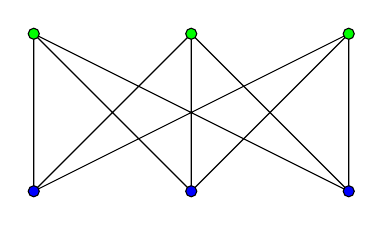
\begin{tikzpicture}
	\tikzstyle{every node}=[circle, draw, inner sep=0pt, minimum width=4pt]
	
	
	\draw (-2, -2) -- (0, 0) -- (0, -2) -- (-2, 0) -- (-2, -2) -- (2, 0) -- (2, -2) -- (-2, 0);
	\draw (0, 0) -- (2, -2);
	\draw (0, -2) -- (2, 0);
    
    \draw (-2, -2) node [fill=blue] {}
    	  (0, -2) node [fill=blue] {}
    	  (2, -2) node [fill=blue] {};
    	  
    \draw (-2, 0) node [fill=green] {}
    	  (0, 0) node [fill=green] {}
    	  (2, 0) node [fill=green] {};
\end{tikzpicture}

	\small Рис. \images. Граф $K_{3, 3}$
\end{center}
\end{paracol}
\refstepcounter{images}

\begin{paracol}{2}
$ $
\newline
\begin{center}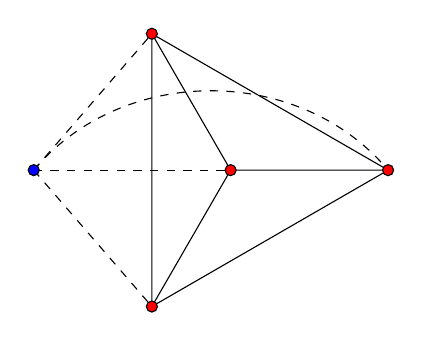
\begin{tikzpicture}
	\tikzstyle{every node}=[circle, draw, fill=red, inner sep=0pt, minimum width=4pt]
	
	\draw (-2.5,0) edge [dashed] (120: 2);
	\draw (-2.5,0) edge [dashed] (0,0);
	\draw (-2.5,0) edge [dashed] (240: 2);
	\draw (-2.5,0) edge [dashed, bend left=50] (0: 2);

	\draw (-2.5,0) node [fill=blue] {};		
	
	\draw \foreach \x in {0,120,240}
    {
    	(\x:2) -- (\x+120:2) -- (0, 0)
    };
    \draw \foreach \x in {0,120,240}
    {
    	(\x:2) node {}
    };
    \draw (0,0) node {};
    
\end{tikzpicture}

	\small Рис. \images. Граф $K_4$ и еще одна вершина
\end{center}
	
\switchcolumn

	Возвращаясь к $K_5$, его непланарность можно получить еще более простыми методами. Достаточно заметить, что в графе 
	$K_4$ каждая грань будет окружена треугольником~---~а значит, кинув на плоскость пятую вершину, мы не сможем ее 
	соединить с какой-то из вершин без пересечения ребер.
	
	Итак, мы разобрали два базовых непланарных графа и теперь можем приступить к формулировке критериев непланарности графов.
\end{paracol}

\mysubsection{Теорема Куратовского и теорема Вагнера}
	
	В прошлом параграфе мы познакомились с первым морфизмом, теперь надо прибегнуть к изучению гомеоморфизма
	
\begin{definition}
	Будем говорить, что граф $G'(V', E')$ получен \emph{делением ребра $e = \lbrace a, b\rbrace$ графа $G(V, E)$}, 
	если он совпадает  ним везде, кроме ребра $e$, вместо которого у него есть два ребра $\lbrace a, c\rbrace$ и $\lbrace c, b\rbrace$.
	
	Граф $G'$ называется \emph{расширением графа $G$}, если он получен засчет деления ребер этого графа.
\end{definition}

\begin{definition}
	Графы $G_1$ и $G_2$ \emph{гомеоморфны}, если существует граф $G_3$, который является расширением обоих графов.
\end{definition}

\begin{center} \;\ \;\ \;\ \;\ \;\ \;\ \;\ \;\ 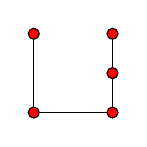
\begin{tikzpicture}
	\tikzstyle{every node}=[circle, draw, fill=red, inner sep=0pt, minimum width=4pt]
	
	\draw (0, 1) -- (0, 0) -- (1, 0) -- (1, 1);
    
    \draw (0, 1) node {}
    	  (0, 0) node {}
    	  (1, 0) node {}
    	  (1, 1) node {}
    	  (1, 0.5) node {};
\end{tikzpicture} \;\ \;\ \;\ \;\ \;\ \;\ 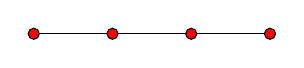
\begin{tikzpicture}
	\tikzstyle{every node}=[circle, draw, fill=red, inner sep=0pt, minimum width=4pt]
	
	\draw (-1, 0) -- (0, 0) -- (1, 0) -- (2, 0);
    
    \draw (-1, 0) node {}
    	  (0, 0) node {}
    	  (1, 0) node {}
    	  (2, 0) node {};
\end{tikzpicture} \;\ \;\ \;\ \;\ \;\ \;\ 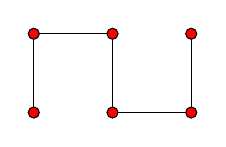
\begin{tikzpicture}
	\tikzstyle{every node}=[circle, draw, fill=red, inner sep=0pt, minimum width=4pt]
	
	\draw (0, -1) -- (0, 0) -- (1, 0) -- (1, -1) -- (2, -1) -- (2, 0);
    
    \draw (0, -1) node {}
    	  (0, 0) node {}
    	  (1, 0) node {}
    	  (1, -1) node {}
    	  (2, -1) node {}
    	  (2, 0) node {};
\end{tikzpicture}
\newline
\newline
	\small Рис. \images. Три гомеоморфных графов
\end{center}

	Как можно видеть на рисунке выше, все графы $P_n$ гомеоморфны при $n \geqslant 2$.
	
	С помощью сравнения степенных последовательностей можно легко сказать, что графы не гомеоморфны, 
	так как в ином случае у них степенные последовательности должны отличаться только числом двоек. Дальше мы даже воспользуемся этим.

	Теперь мы можем сформулировать первый критерий.
	
\begin{theorem}[Понтрягина-Куратовского]
	Граф $G$ планарен тогда и только тогда, когда не содержит подграфа, гомеоморфного $K_{3, 3}$ и $K_5$.
\end{theorem}

	К сожалению, эта и следующая теоремы из списка тех, которые имеют довольно простую формулировку, 
	но доказательство у них не элементарно ни в коем роде, так что оставим его до лучших времен.

\begin{definition}
	Будем говорить, что граф $G'$ получен из графа $G$ \emph{стягиванием ребра $e = \lbrace a, b\rbrace$}, 
	если вместо этих двух вершин в нем одна вершина $c$, которая смежна с теми вершинами, с которыми была 
	смежна хотя бы одна вершина: $a$ или $b$. Обозначение: $G/e$.
\end{definition}

\begin{definition}
	Граф $G'$ называется \emph{минором графа $G$}, если он может быть получен из него посредством стягивания ребер и удаления ребер и вершин.
\end{definition}

\begin{theorem}[Вагнера]
	Граф $G$ планарен тогда и только тогда, когда он не содержит минора, изоморфного $K_{3, 3}$ или $K_5$.
\end{theorem}

\begin{paracol}{2}
	
\begin{example}
	Ранее я уже приводил рисунок графа Петерсена, который в свое время стал популярным из-за своей непланарности.
	
	Его непланарность можно доказать по обоим теоремам. Для доказательства через теорему
	Вагнера достаточно стянуть пять ребер, обозначенных на рисунке ниже слева, и получить $K_5$. 
	А для теоремы Понтрягина-Куратовского нужно построить вручную подграф, гомеоморфный $K_{3, 3}$.
\end{example}

\switchcolumn

\begin{center}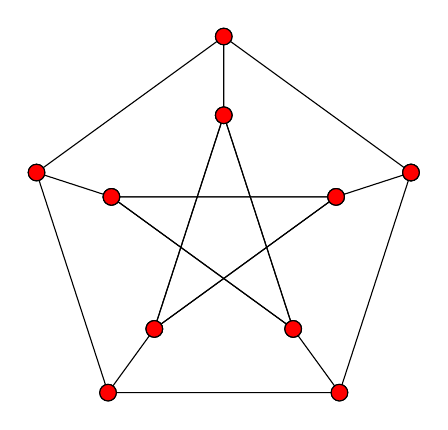
\begin{tikzpicture}
	\tikzstyle{every node}=[circle, draw, fill=red, inner sep=0pt, minimum width=6pt]
	\foreach \x in {18,90,...,306}
    {
    	\draw
    	(\x:1.5) node {} -- (\x+144:1.5)
    	(\x:1.5) node {} -- (\x+216:1.5);
    };
    \foreach \x in {18,90,...,306}
    {
    	\draw
    	(\x:2.5) node {} -- (\x:1.5)
    	(\x:2.5) node {} -- (\x+72:2.5);
    };
    \draw \foreach \x in {18,90,...,306}
    {
    	(\x:1.5) node {}
    };
    \draw (18: 2.5) node {};
\end{tikzpicture}\end{center}
\begin{center}
	\small Рис. \images. Графа Петерсена
\end{center}
\end{paracol}
\refstepcounter{images}

\begin{center}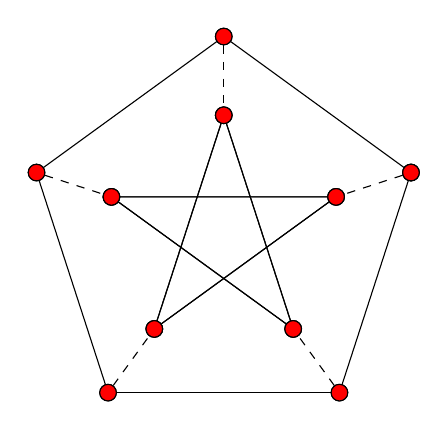
\begin{tikzpicture}
	\tikzstyle{every node}=[circle, draw, fill=red, inner sep=0pt, minimum width=6pt]
	\foreach \x in {18,90,...,306}
    {
    	\draw
    	(\x:1.5) node {} -- (\x+144:1.5)
    	(\x:1.5) node {} -- (\x+216:1.5);
    };
    \foreach \x in {18,90,...,306}
    {
    	\draw
    	(\x:2.5) node {} edge [dashed] (\x:1.5)
    	(\x:2.5) node {} -- (\x+72:2.5);
    };
    \draw \foreach \x in {18,90,...,306}
    {
    	(\x:1.5) node {}
    };
    \draw (18: 2.5) node {};
    
\end{tikzpicture} \;\ \;\ \;\ \;\ \;\ \;\ \;\ 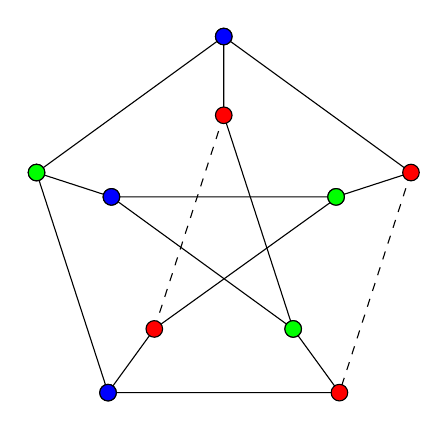
\begin{tikzpicture}
	\draw (90: 1.5) edge [dashed] (234: 1.5)
		  (18: 2.5) edge [dashed] (306: 2.5);
    
	\draw (162: 2.5) -- (90: 2.5)
		  (162: 2.5) -- (162: 1.5)
		  (162: 2.5) -- (234: 2.5);    
    
	\draw (18: 1.5) -- (18: 2.5) -- (90: 2.5)
		  (18: 1.5) -- (162: 1.5)
		  (18: 1.55) -- (234: 1.5) --(234: 2.5);    
    
	\draw (306: 1.5) -- (90: 1.5) -- (90: 2.5)
		  (306: 1.5) -- (162: 1.5)
		  (306: 1.5) -- (306: 2.5) --(234: 2.5);    
	
	\tikzstyle{every node}=[circle, draw, fill=red, inner sep=0pt, minimum width=6pt]

    \draw \foreach \x in {18,90,...,306}
    {
    	(\x:1.5) node {}
    	(\x:2.5) node {}
    };
    
    \tikzstyle{every node}=[circle, draw, fill=green, inner sep=0pt, minimum width=6pt]
    
    \draw (18: 1.5) node {}
    	  (162: 2.5) node {}
    	  (306: 1.5) node {};
   
    \tikzstyle{every node}=[circle, draw, fill=blue, inner sep=0pt, minimum width=6pt]
    
    \draw (90: 2.5) node {}
    	  (162: 1.5) node {}
    	  (234: 2.5) node {};
\end{tikzpicture}\end{center}
\begin{center}
	\small Рис. \images. Графа Петерсена: с изображенными ребрами, по которым надо его стягивать, 
	чтобы получить $K_5$ (слева); с изображенным подграфом, гомеоморфном $K_{3, 3}$ (справа)
\end{center}

	Ранее мне рассказали такую интересную историю: на ФУПМе в $4$ семестре читается курс АМВ. 
	На контрольной по этой дисциплине дали задачу: доказать непланарность графа Петерсена, при этом 
	во время лекций не упоминали про теорему Вагнера. Все, без исключения, сказали, что этот граф непланарен 
	в силу того, что в нем есть гомеоморф $K_5$. 
	
	Это ложь! Как минимум, мы уже сказали про отличия в степенных последовательностях гомеоморфных графов. 
	В графе Петерсена нет вершин со степенью, равной четырем, а в $K_5$ все вершины с такой степенью.
	
\mysubsection{Интересные факты}

	В некоторых задачах можно наткнуться на понятие выпуклой оболочки. Как таковое, оно не входит в теорию графов, 
	однако полезно знать о нём и в некоторых задачах использовать.
	
	Допустим, что на плоскости отмечено произвольное (конечное) число точек. Тогда существует такой выпуклый многоугольник 
	с вершинами в некоторых отмеченных точках, что все остальные точки лежат внутри него. Этот многоугольник и называется \emph{выпуклой оболочкой}.
	
\begin{center}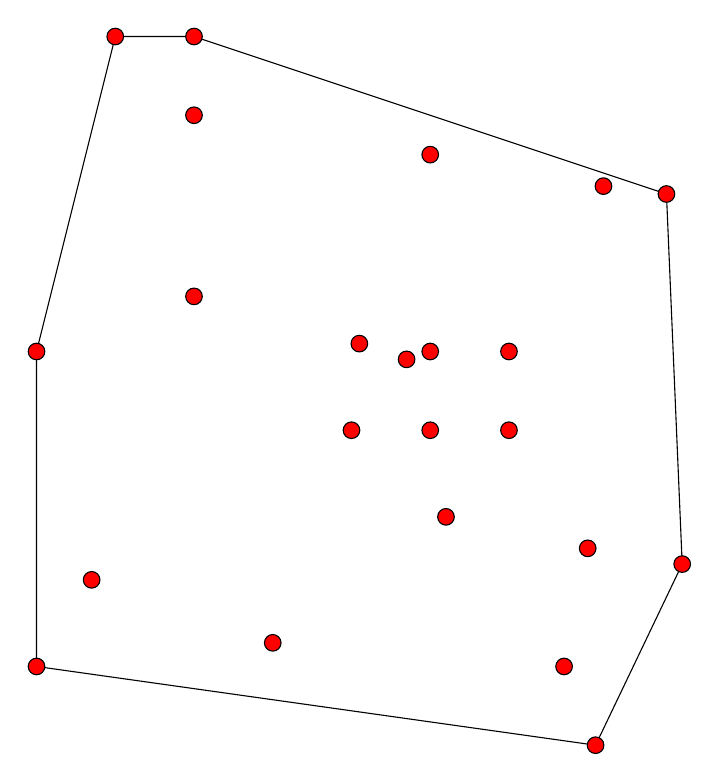
\begin{tikzpicture}
	\tikzstyle{every node}=[circle, draw, fill=red, inner sep=0pt, minimum width=6pt]

	\draw (-4, -4) -- (-4, 0) -- (-3, 4) -- (-2, 4) -- (4, 2) -- (4.2, -2.7) -- (3.1, -5) -- (-4, -4);

    \draw (1, 2.5) node {};
    \draw (2.7, -4) node {};
    \draw (3.1, -5) node {};
    \draw (-2, 3) node {};
    \draw (4, 2) node {};
    \draw (-3, 4) node {};
    \draw (-2, 4) node {};
    \draw (3, -2.5) node {};
    \draw (-4, -4) node {};
    \draw (-3.3, -2.9) node {};
    \draw (3.2, 2.1) node {};
    \draw (0.1, 0.1) node {};
    \draw (0.7, -0.1) node {};
    \draw (1.2, -2.1) node {};
    \draw (0, -1) node {}
    	  (1, 0) node {}
    	  (1, -1) node {}
    	  (2, -1) node {}
    	  (2, 0) node {};
    \draw (-4, 0) node {};
    \draw (-2, 0.7) node {};
    \draw (-1, -3.7) node {};
    \draw (4.2, -2.7) node {};
    	  
\end{tikzpicture}\end{center}
\begin{center}
	\small Рис. \images. Произвольное множество точек плоскости с их выпуклой оболочкой
\end{center}

	Планарные графы по определению можно изобразить на плоскости без самопересечения рёбер. Оказывается, что 
	все планарные графы можно с тем же условием нарисовать и на сфере. Кроме того, обратное утверждение верно, 
	то есть любой конечный граф на сфере можно изоморфно переместить в граф на плоскости.

\begin{paracol}{2}
\begin{center}\begin{tikzpicture} % "THE GLOBE" showcase

\def\R{2.5}; % sphere radius
\def\angEl{35}; % elevation angle
\def\angAz{-105}; % azimuth angle
\def\angPhi{40}; % longitude of point P
\def\angBeta{-10}; % latitude of point P

%% working planes

\pgfmathsetmacro\H{\R*cos(\angEl)}; % distance to north pole
\tikzset{xyplane/.style={cm={cos(\angAz),sin(\angAz)*sin(\angEl),-sin(\angAz),
                              cos(\angAz)*sin(\angEl),(0,-\H)}}};
\LongitudePlane[xzplane]{\angEl}{\angAz};
\LongitudePlane[pzplane]{\angEl}{\angPhi};
\LatitudePlane[equator]{\angEl}{0};

%% draw xyplane and sphere

\draw[xyplane] (-1*\R,-1*\R) rectangle (1.1*\R,1.8*\R);
\fill[ball color=white] (0,0) circle (\R); % 3D lighting effect
\draw (0,0) circle (\R);

%% characteristic points

\coordinate (O) at (0,0);
\coordinate[mark coordinate] (N) at (0,\H);
\coordinate[mark coordinate] (S) at (0,-\H);
\path[pzplane] (\angBeta:\R) coordinate[mark coordinate] (P);
\path[pzplane] (\R,0) coordinate (PE);
\path[xzplane] (\R,0) coordinate (XE);
\path (PE) ++(0,-\H) coordinate (Paux); % to aid Phat calculation

\coordinate[mark coordinate] (Phat) at (intersection cs: first line={(N)--(P)}, second line={(S)--(Paux)});

%% draw meridians and latitude circles

\DrawLatitudeCircle[\R]{0} % equator
%\DrawLatitudeCircle[\R]{\angBeta}
\DrawLongitudeCircle[\R]{\angAz} % xzplane
\DrawLongitudeCircle[\R]{\angAz+90} % yzplane
\DrawLongitudeCircle[\R]{\angPhi} % pzplane

%% draw xyz coordinate system

%\draw[xyplane,<->] (1.8*\R,0) node[below] {$x,\xi$} -- (0,0) -- (0,2.4*\R)
%    node[right] {$y,\eta$};
%\draw[->] (0,-\H) -- (0,1.6*\R) node[above] {$z,\zeta$};

%% draw lines and put labels

\draw[dashed] (P) -- (N) +(0.3ex,0.9ex) node[above left] {$\mathbf{N}$};
\draw (P) -- (Phat) node[above right] {$\mathbf{\hat{P}}$};
\draw (P) node[above right] {$\mathbf{P}$};
\end{tikzpicture}

	\small Рис. \images. Сферическая проекция
\end{center}

\switchcolumn

	Чтобы убедить вас в том, что любой многогранник можно поместить в плоскость без самопересечений ребер, 
	хочу обратить ваше внимание на рисунок слева. На нем показана сферическая проекция на плоскость, 
	которая переводит все связанные линие в связанные. Пользуясь ей можно провернуть и обратную операцию~---~а 
	именно, переместить плоский граф на сферу.
	
$ $
\newline
	Итак, мы познакомились с планарными графами. Сформулировали два критерия планарности графов и посмотрели 
	под разными углами на граф Петерсена.
\end{paracol}
	
\mysubsection{Задачи}

\begin{exersize}
	В некоторой стране есть $n$ озер, которые соединены $k$ каналами. Из любого озера по каналам можно добраться 
	в любое другое озеро. Сколько в этой стране островов?
\end{exersize}

\begin{exersize}[Канель-Белов А.Я., Ковальджи А.К. Как решают нестандартные задачи]
	На плоскости дано $n$ точек, соединенных непересекающимися отрезками. Может ли оказаться так, 
	что каждая точка будет соединена ровно с шестью другими?
\end{exersize}

\begin{exersize}
	На плоскости отмечено несколько точек, никакие три из которых не лежат на одной прямой. Двое по очереди соединяют 
	отрезком две какие угодно еще не соединенные точки так, чтобы отрезки не пересекались нигде, кроме отмеченных точек. 
	Проигрывает тот, кто не сможет сделать ход. Докажите, что один из играющих будет всегда выигрывать независимо от своей игры и игры соперника.
\end{exersize}

\begin{exersize}
	Один из простейших многоклеточных организмов~---~водоросль <<вольвокс>>~---~представляет собой сферическую оболочку, 
	сложенную семиугольными, шестиугольными и пятиугольными клетками (в каждой <<вершине>> сходятся три клетки). 
	Биологи заметили, что пятиугольных клеток всегда ровно на 12 больше, чем семиугольных (всего клеток может быть несколько сотен и даже тысяч). 
	Не можете ли вы объяснить этот странный факт?
\end{exersize}

\begin{exersize}
	Пусть все грани выпуклого многогранника~---~правильные $n$-угольники, и в каждой его вершине сходится ровно $k$ граней. 
	Докажите, что тогда $\frac{1}{n} + \frac{1}{k} = \frac{1}{2} + \frac{1}{r}$, где $r$~---~число его рёбер.
\end{exersize}

